% Chapter Template

% Main chapter title
\chapter{Tokenizer Adaptation}

% Short version of the title for the header
\chaptermark{Tokenizer Adaptation}

% Chapter Label
\label{chap:tokenizer_adaptation}

This chapter presents the methodological framework for adapting existing language models to new target languages with minimal retraining. The central idea of this thesis—“Hacking the Tokenizer”—is to exploit the tokenizer as the main adaptation point, allowing pre-trained models to process new languages by extending their vocabulary rather than retraining the entire model. 

Recent work \cite{kim2025finetune} demonstrates that extending tokenizers with domain-specific tokens can improve fine-tuning efficiency, which motivates our decision to carefully curate the Portuguese vocabulary extension

Our case study focuses on European Portuguese (PT-PT). This language was selected both because it is our native language and the target audience of this work, and also because its orthographic and morphological characteristics pose interesting challenges for tokenizer adaptation. This makes it a strong test case for evaluating the effectiveness of tokenizer-level adaptation.

The overall workflow follows three stages:
\begin{enumerate}
    \item Selecting which new tokens to add to the vocabulary (\S\ref{sec:token_selection}).
    \item Initializing embeddings for these tokens (\S\ref{sec:embedding_init}).
    \item Optionally fine-tuning embeddings with lightweight training (\S\ref{sec:embedding_finetune}).
\end{enumerate}

This chapter details each of these stages and prepares the ground for the inference adaptation in Chapter~\ref{chap:inference_adaptation} and results in Chapter~\ref{chap:results}.

% --------------------------------------------------------------
\section{Experimental Setup}
\label{sec:exp_setup}

All experiments reported in this thesis used the following configuration unless otherwise noted:
\begin{itemize}
    \item \textbf{Models:} SmolLM2-135M (monolingual), Qwen2.5-1.5B-Instruct (multilingual) and SmolLM3-3B (multilingual).
    \item \textbf{Tokenizers:} (BPE) with initial vocabulary sizes of  $\approx 50,000$, $\approx 150,000$ and $\approx 130,000$.
    \item \textbf{Portuguese Corpus:} OpenSubtitles\footnote{OpenSubtitles Corpus: \url{https://opus.nlpl.eu/results/en&pt/corpus-result-table}}, restricted to European Portuguese (PT-PT) entries.
    \item \textbf{Evaluation Benchmarks:} CalamePT (\S\ref{subsec:dataset-calamept}) and SuperGluePTPT (\S\ref{subsec:dataset-superglueptpt}), detailed in Chapter~\ref{chap:results}.
\end{itemize}

% --------------------------------------------------------------
\section{Token Selection Methodology}
\label{sec:token_selection}

The first step in adapting a model to a new language is identifying which tokens to add. Tokenizer design choices such as vocabulary size, training corpus, and pre-tokenization regular expressions can significantly impact downstream model performance \cite{dragan2024mosttoken}.

To adapt SmolLM2-135M for Portuguese, we expanded the vocabulary by up to 10,000 tokens using the \texttt{add\_tokens}\footnote{HuggingFace \href{https://huggingface.co/docs/transformers/v4.56.1/en/main\_classes/tokenizer\#transformers.PreTrainedTokenizer.add\_tokens}{documentation}} functionality of the Hugging Face Transformers library. The procedure was:

\begin{itemize}
    \item Train a new BPE tokenizer with a target vocabulary size of $2 \times size$, where $size$ is the number of tokens to be added.
    \item Remove all tokens already present in the original vocabulary.
    \item Remove tokens that are substrings of existing tokens (e.g., discard \textit{pub} if \textit{público} is already in the vocabulary).
    \item Rank the remaining tokens by frequency of occurrence in the Portuguese corpus.\footnote{Here, frequency is defined as the number of times a token appears in the training corpus.}
    \item Select the top $size$ tokens for integration.
\end{itemize}

This pipeline ensures that the expansion captures Portuguese-specific tokens with high frequency and utility while minimizing redundancy with the original tokenizer. For example, words like \textit{chegada} (arrival), \textit{trabalhar} (to work), or \textit{rapidamente} (quickly) frequently appear in Portuguese but are fragmented into multiple subtokens by the original tokenizer; they become strong candidates for inclusion.

% \textit{Transition: Having identified a list of useful new tokens, the next step is to initialize their embeddings so that they integrate smoothly into the model’s vector space.}

% --------------------------------------------------------------
\section{Embedding Initialization Strategies}
\label{sec:embedding_init}

When extending the vocabulary, each new token must be assigned an embedding vector. Poor initialization can lead to embeddings that are semantically inconsistent with the rest of the model, degrading performance.

\subsection{Baseline Methods}
Most prior work expands vocabularies using simple strategies such as:
\begin{itemize}
    \item \textbf{Random Initialization:} New embeddings are sampled from the same distribution used during model training \cite{kocmi2017embed}.
    \item \textbf{Cross-Lingual Mapping:} Embeddings are mapped from a source language to a target language space using bilingual lexicons or alignment methods. For example, Singh \cite{singh2025tokeninit} leverages statistical word alignment (via GIZA++) to construct initialization matrices for new tokens, while Minixhofer \cite{minixhofer2022subwembedinit} proposes WECHSEL, which aligns new embeddings with semantically similar embeddings from another language. These methods have shown strong results in multilingual adaptation but require parallel corpora or high-quality multilingual resources.
    \item \textbf{Heuristic Initialization:} More lightweight methods directly exploit information from the model's existing embedding space. Dobler \cite{dobler2023embedinit} propose FOCUS, which represents new tokens as weighted combinations of existing embeddings, while Liu \cite{liu2024embedinit} introduce OFA, a framework that injects knowledge from external multilingual word vectors into the embedding matrix. Although effective, both methods rely on auxiliary models or external vector spaces.
\end{itemize}


While these approaches have proven effective in some scenarios, they often require additional resources such as bilingual dictionaries, parallel corpora, or multilingual static embeddings, and sometimes involve further training stages. Since our work explicitly targets low-resource and minimal-retraining scenarios, we instead focused on lightweight alternatives that can be applied even when no bilingual resources are available.

\subsection{Mean Vector Initialization}
\label{subsec:mean-init}
The first approach, termed "Mean Vector Initialization", computes the embedding for each new token by averaging the embeddings of its constituent subtokens as determined by the original tokenizer, as shown in Figure~\ref{fig:mean-init}.


\begin{figure}[ht]
\centering
\begin{tikzpicture}
\node at (0,0) {$E(T_{\text{new}}) = \left[ \frac{S_1}{n}, \frac{S_2}{n}, \dots, \frac{S_N}{n} \right]$};
\matrix (tokens) [matrix of math nodes,
    nodes={draw, minimum width=2.5em, minimum height=2em},
    row sep=1em, column sep=0.2em,
    below=of {(0,0)}
] {
    T_1 & T_2 & T_3 & \dots & T_n \\
};
\matrix (embeddings) [matrix of math nodes,
    nodes={draw, minimum width=3em, minimum height=2em},
    below=2em of tokens,
    column sep=0.2em, row sep=0.1em
] {
  E_{1,1} & E_{1,2} & E_{1,3} & \dots & E_{1,N} \\
  + & + & + & + & + \\
  E_{2,1} & E_{2,2} & E_{2,3} & \dots & E_{2,N} \\
  + & + & + & + & + \\
  \vdots & \vdots & \vdots & \ddots & \vdots \\
  + & + & + & + & + \\
  E_{n,1} & E_{n,2} & E_{n,3} & \dots & E_{n,N} \\
};
\matrix (sums) [matrix of math nodes,
    nodes={draw, minimum width=3em, minimum height=2em},
    below=2em of embeddings,
    column sep=0.2em
] {
  \sum_{i=1}^n E_{i,1} & \sum_{i=1}^n E_{i,2} & \sum_{i=1}^n E_{i,3} & \dots & \sum_{i=1}^n E_{i,N} \\
};
\node[left=0.5em of sums-1-1] (slabel) {$S = $};
\end{tikzpicture}
\caption{Mean Vector Initialization: Averaging subtoken embeddings with summation}
\label{fig:mean-init}
\end{figure}

After computing the embeddings for all new tokens, the model's embedding matrix was extended by assigning:
\begin{verbatim}
model.embeddings.weight[new_token_id] = new_embedding_vector
\end{verbatim}

This method provides a straightforward approach that captures the average semantic content of the constituent tokens. The intuition is that the meaning of a compound token can be approximated by the average meaning of its parts. For example, the Portuguese word "chegada" might be tokenized as "che" + "gada" in the original tokenizer, and the embedding for the new single token "chegada" would be the average of the embeddings for "che" and "gada".

Although this approach is computationally efficient and intuitive, it treats all constituent tokens as equally important to the semantic meaning of the compound token, which may not always be the case in morphologically rich languages.


\subsection{Position-Weighted Initialization}
\label{subsec:pos-wei-init}

The second approach, termed "Position-Weighted Initialization", assigns differential importance to constituent tokens based on their position within the sequence. This method is predicated on the hypothesis that initial tokens in a sequence typically carry greater semantic significance in autoregressive language models.

For a new token decomposed into the sequence $(t_1, t_2, \ldots, t_n)$ by the original tokenizer, weights are assigned such that:



$$
\begin{array}{c}
    \text{Let } new\_token = (t_1, t_2, \ldots, t_n) \\
    E(new\_token) = \frac{\sum_{i=1}^{n} w_i \times E(t_i)}{\sum_{i=1}^{n} w_i} \\
    \text{where } w_i = K^{n-i} \text{ for } i \in \{1,2,\ldots,n\}
\end{array}
$$
\unsure{ADD Diagram here showcasing the "Position-weighted" method.}

The parameter $K > 1$ determines the degree of positional bias, with higher values of $K$ placing greater emphasis on earlier tokens. This approach was motivated by the observation that autoregressive models typically assign higher predictive importance to initial tokens in a sequence.

For example, with $K = 1.5$ and a token decomposed into three subtokens, the weights would be approximately:
\begin{itemize}
    \item $w_1 = 1.5^2 = 2.25$ (first token)
    \item $w_2 = 1.5^1 = 1.5$ (second token)
    \item $w_3 = 1.5^0 = 1.0$ (third token)
\end{itemize}

All these weights are then normalized to sum to 1, resulting in:
\begin{itemize}
    \item $w_1 = \frac{2.25}{2.25+1.5+1} \approx 0.47$
    \item $w_2 = \frac{1.5}{2.25+1.5+1}  \approx 0.32$
    \item $w_3 = \frac{1}{2.25+1.5+1}    \approx 0.21$
\end{itemize}

This weighting scheme ensures that the first token contributes more than twice as much to the final embedding as the last token, reflecting its greater importance in determining the semantic meaning of the compound token.

% --------------------------------------------------------------
\section{Comparative Analysis of Initialization Methods}

We conducted extensive experiments to compare the effectiveness of these initialization strategies, including various values of the weighting parameter $K$ for the Position-Weighted Initialization method.

\subsection{Evaluation Methodology}
\label{subsec:evaluation_methodology}

To ensure a fair comparison across initialization strategies, we designed a controlled evaluation pipeline that focuses on the predictive ability of new tokens introduced into the vocabulary. The procedure was as follows:

\begin{enumerate}
    \item A list of Portuguese-specific tokens (\texttt{new\_tokens}) was generated from the BPE tokenizer trained on the \texttt{OpenSubtitlesPT} subset (see \S\ref{sec:token_selection}).
    \item For each initialization method, the base model was modified to include the \texttt{new\_tokens} and corresponding embeddings.
    \item From the \texttt{OpenSubtitlesPT} corpus, we sampled 1,000 lines containing at least one of the \texttt{new\_tokens}.
    \item For each line:
        \begin{enumerate}
            \item Randomly select one \texttt{new\_token} present in the line.
            \item Split the line at that token, discarding the final fragment (i.e., keep \texttt{phrase.split(token)[:-1]}).
            \item Use \texttt{model.generate} to continue the text from the remaining fragments.
            \item Record the model's predicted logits and the rank of the correct \texttt{new\_token} among all vocabulary candidates.
        \end{enumerate}
    \item Repeat until all sampled lines have been processed.
\end{enumerate}

This methodology directly evaluates how well each initialization strategy positions new embeddings in the model's vector space, as measured by the model’s ability to correctly predict unseen tokens in realistic contexts. It also allows us to compare methods under consistent conditions without additional fine-tuning or external resources.



\subsection{Results}
\label{subsec:results}

Using the evaluation methodology described in \S\ref{subsec:evaluation_methodology}, we compared all embedding initialization strategies by counting, for each method, the number of times it achieved the best (i.e., lowest) rank for a new token across 1,000 sampled lines. This metric directly reflects the model’s ability to correctly predict unseen tokens given partial context.

The aggregated results are summarized in Table~\ref{tab:embed_init_results}. Among the tested methods, the Position-Weighted Initialization variants generally outperformed the baseline strategies. Specifically, \texttt{weighted\_drop(5.0)} achieved the highest number of wins (127), followed closely by \texttt{weighted\_drop(4.5)} (126). However, extreme weighting values tend to place excessive emphasis on the first subtoken, which can distort the semantic representation of longer tokens and potentially degrade generalization.

\begin{table}[ht]
    \centering
    \begin{tabular}{l c}
        \toprule
        Initialization Method & Number of Wins \\
        \midrule
        Random Initialization & 36 \\
        Mean Vector Initialization & 39 \\
        Weighted Drop (K=0.5) & 26 \\
        Weighted Drop (K=1.0) & 37 \\
        Weighted Drop (K=1.5) & 47 \\
        Weighted Drop (K=2.0) & 53 \\
        Weighted Drop (K=2.5) & 81 \\
        Weighted Drop (K=3.0) & 89 \\
        Weighted Drop (K=3.5) & 79 \\
        Weighted Drop (K=4.0) & 99 \\
        Weighted Drop (K=4.5) & 126 \\
        Weighted Drop (K=5.0) & 127 \\
        \bottomrule
    \end{tabular}
    \caption{Number of times each method achieved the lowest rank across 1,000 sampled lines. Minimum and lower-quartile values are omitted from this table due to their likely outlier behavior.}
    \label{tab:embed_init_results}
\end{table}

It is worth noting that some metrics, such as the minimum and first quartile for certain weighted variants, were observed to be higher (worse) than expected. These extreme values likely reflect outlier cases in the evaluation data and are not considered in the main comparison, as they do not represent typical performance\footnote{For example, some \texttt{weighted\_drop} variants occasionally produced unusually poor predictions for specific tokens due to the extreme weighting of the first subtoken. These cases were rare and do not affect the overall trend.}.

Despite \texttt{weighted\_drop(5.0)} achieving the highest number of wins, we selected \texttt{weighted\_drop(1.5)} as our default initialization strategy. This choice strikes a balance between emphasizing the first subtoken and preserving semantic contributions from later subtokens. It consistently outperformed baseline methods while avoiding the potential distortions introduced by extreme weighting, aligning with our goal of low-cost, minimal-retraining adaptation.

These findings reinforce the importance of positional weighting in embedding initialization and provide a principled foundation for all downstream evaluations in subsequent chapters.




% --------------------------------------------------------------
\section{Embedding Fine-tuning}
\label{sec:embedding_finetune}

In addition to initialization, we implemented a lightweight, context-aware fine-tuning procedure to further refine embeddings of the new tokens. The key idea is to update only the embeddings of the newly added tokens while leaving the rest of the model frozen. This ensures minimal interference with the pretrained knowledge. 

For each new token, we extract phrases from the training dataset that precede the token and discard the trailing fragment. We then run the model in generation mode to compute logits and hidden states for these phrases. The embedding for the target token is updated proportionally to the difference between the maximum predicted logit and the logit corresponding to the token, using the last hidden state of the generation as a directional signal.  

This procedure can be summarized as follows:
\begin{itemize}
    \item \textbf{Training Objective:} Context-aware embedding refinement for new tokens using generated logits and hidden states.
    \item \textbf{Frozen Parameters:} All model weights except the embeddings of the new tokens.
    \item \textbf{Data:} Corpus of CalamePT\footnote{Although using this corpus could theoretically introduce bias, the fine-tuning produced no measurable performance gains, so the dataset was retained.}.
    \item \textbf{Batching:} Phrases are processed in batches for computational efficiency.
    \item \textbf{Training Budget:} A single pass through the dataset with a small learning rate, significantly cheaper than full model fine-tuning.
\end{itemize}

This approach nudges the new embeddings toward vector representations that better align with the model's predictions in realistic contexts while preserving the pretrained model's original knowledge. Importantly, empirical evaluation showed that this procedure produced no significant bias, as measured by downstream performance metrics.




\section{Chapter Summary and Rationale for Method Selection}

In this chapter, we presented a systematic approach for adapting pre-trained language models to a new target language by “hacking” the tokenizer. The process involved three key stages: (1) selecting high-utility new tokens from a Portuguese corpus, (2) initializing embeddings for these tokens using both baseline and novel strategies, and (3) optionally fine-tuning the new embeddings with lightweight training. 

Our experimental analysis demonstrated that the choice of embedding initialization has a significant impact on the model’s ability to predict new tokens. Among the strategies tested, the Position-Weighted Initialization with extreme weighting (\texttt{weighted\_drop(5)}) achieved the highest number of wins in terms of predictive rank. However, this approach overemphasizes the first subtoken, potentially neglecting semantic contributions from subsequent subtokens.

To balance positional bias with semantic fidelity, we selected \texttt{weighted\_drop(1.5)} as our default initialization strategy for all further experiments. This variant provides a moderate weighting scheme that preserves the importance of the initial subtoken while still incorporating information from later subtokens. When combined with the lightweight fine-tuning procedure, it further refines new token embeddings without altering the pretrained model’s knowledge. This strategy consistently outperformed baseline methods, aligning with our goal of low-cost, minimal-retraining adaptation. 

By standardizing on \texttt{weighted\_drop(1.5)} and applying optional embedding fine-tuning, we establish a consistent and principled foundation for all downstream evaluations presented in subsequent chapters.
































% OLD CHAPTER HERE IN CASE I WANT TO ROLL BACK









% % Chapter Template

% % Main chapter title
% \chapter{Tokenizer Adaptation}

% % Short version of the title for the header
% \chaptermark{TokenizerAdaptation}

% % Chapter Label
% \label{chap:tokenizer_adaptation}

% % Write text in here
% This chapter presents the methodological framework for adapting existing language models to new target languages with minimal retraining. The central idea of this thesis—“Hacking the Tokenizer”—is to exploit the tokenizer as the main adaptation point, allowing pre-trained models to process new languages by extending their vocabulary rather than retraining the entire model. 

% Recent work \cite{kim2025finetune} demonstrates that extending tokenizers with domain-specific tokens can improve fine-tuning efficiency, which further motivates our decision to carefully curate the Portuguese vocabulary extension.

% Our case study focuses on European Portuguese. This language was selected both because it is our native language and the target audience of this work, and also because its orthographic and morphological characteristics pose interesting challenges for tokenizer adaptation. This makes it a strong test case for evaluating the effectiveness of tokenizer-level adaptation.

% The overall workflow follows three stages:
% \begin{enumerate}
%     \item Selecting which new tokens to add to the vocabulary (\S\ref{sec:token_selection}).
%     \item Initializing embeddings for these tokens (\S\ref{sec:embedding_init}).
%     \item Optionally fine-tuning embeddings with lightweight training (\S\ref{sec:embedding_finetune}).
% \end{enumerate}

% This chapter walks through each of these stages, presents different strategies, and compares their effectiveness on benchmark tasks. 


% \section{Token Selection Methodology}
% \label{sec:token_selection}

% The first step in adapting a model to a new language is identifying which tokens to add. The selection must be principled: arbitrary additions risk redundancy and inefficiency. The guiding principle is to replicate the algorithm of the original tokenizer, so that the extended vocabulary remains consistent with the model's original design.

% Most of our experiments used the \textit{HuggingFaceSmolLm135M} model, whose tokenizer has a vocabulary of roughly 50,000 tokens. To adapt it for Portuguese, we expanded the vocabulary by about 10,000 tokens using the \texttt{added\_tokens} functionality of the Hugging Face Transformers library.\footnote{HuggingFace Transformers: \url{https://huggingface.co/}} 

% Because this model was originally trained with a Byte-Pair Encoding (BPE) tokenizer, we trained a new BPE tokenizer on a Portuguese corpus obtained from OpenSubtitles.\footnote{OpenSubtitles Corpus: \url{https://opus.nlpl.eu/results/en&pt/corpus-result-table}} The following steps were then applied to extract a set of high-utility new tokens:

% \begin{itemize}
%     \item Train a new BPE tokenizer with a target vocabulary size of $2 \times size$, where $size$ is the number of tokens to be added.
%     \item Remove all tokens already present in the original vocabulary.
%     \item Remove tokens that are substrings of existing tokens (e.g., discard \textit{pub} if \textit{público} is already in the vocabulary).
%     \item Rank the remaining tokens by frequency of occurrence in the Portuguese corpus.\footnote{Here, frequency is defined as the number of times a token appears in the training corpus.}
%     \item Select the top $size$ tokens for integration.
    
% \end{itemize}

% This pipeline ensures that the expansion captures Portuguese-specific tokens with high frequency and utility while minimizing redundancy with the original tokenizer. For example, words like \textit{chegada} (arrival), \textit{trabalhar} (to work), or \textit{rapidamente} (quickly) frequently appear in Portuguese but are fragmented into multiple subtokens by the original tokenizer; they become strong candidates for inclusion.

% \textit{Having identified a list of useful new tokens, the next step is to initialize their embeddings so that they integrate smoothly into the model’s vector space.}

% \section{Embedding Initialization Strategies}
% \label{sec:embedding_init}

% When extending the vocabulary, each new token must be assigned an embedding vector. Poor initialization can lead to embeddings that are semantically inconsistent with the rest of the model, resulting in degraded performance. In this section we describe baseline strategies found in prior work and then introduce two novel methods.

% \subsection{Baseline Methods}
% Most prior work expands vocabularies using simple strategies such as:
% \begin{itemize}
%     \item \textbf{Random Initialization:} New embeddings are sampled from the same distribution used during model training \cite{https://arxiv.org/abs/1711.09160}.
%     \item \textbf{Cross-Lingual Mapping:} Embeddings are mapped from a source language to a target language space using bilingual lexicons or alignment methods \cite{all_researches_here}. 
% \end{itemize}

% Although Cross-Lingual Mapping has shown strong results in multilingual adaptation, it typically requires substantial external resources such as bilingual dictionaries or parallel corpora, and often involves an additional training stage. Since our work explicitly targets low-resource and minimal-retraining scenarios, we did not employ this method. Instead, we focused on lightweight alternatives that can be applied even when no bilingual resources are available.


% \subsection{Mean Vector Initialization}
% \label{subsec:mean-init}
% The first approach, termed "Mean Vector Initialization," computes the embedding for each new token by averaging the embeddings of its constituent subtokens as determined by the original tokenizer, as shown in the picture bellow.

% ========================================================================================
% PLACEHOLDER FOR PICTURE SHOWING A DIAGRAM HERE OF MEAN VECTOR INITIALIZATION
% \unsure{How can I make this a Diagram instead? Which software gives me that possibility?}
% $$
% \begin{array}{c}
%     \text{Let } E(t) = \text{Embedding function for token } t \\
%     \forall\, \text{new\_token} \in \text{new\_tokens} \\
%     \text{Let } \text{OldTokenization}(new\_token) = \{t_1, t_2, \ldots, t_n\} \\
%     E(\text{new\_token}) = \frac{1}{n} \sum_{i=1}^{n} E(t_i)
% \end{array}
% $$

% % ----------------------------------------------------------------------------------------
% %                                       OPTION 1
% \begin{figure}[ht]
% \centering
% \begin{tikzpicture}

% % Top: Token concatenation
% \node at (0,0) {$T_{\text{new}} = $};
% \matrix (tokens) [matrix of nodes, nodes={draw, minimum width=1.2em, minimum height=2em}, right=of {0,0}, column sep=0.2em] {
%   $T_1$ & $T_2$ & $T_3$ & $\dots$ & $T_n$ \\
% };

% % Middle: Embedding matrix
% \matrix (embeddings) [matrix of math nodes, nodes={draw, minimum width=2em, minimum height=2em}, below=2 of tokens, column sep=0.2em, row sep=0.2em] {
%   E_{1,1} & E_{1,2} & E_{1,3} & \dots & E_{1,N} \\
%      +    &    +    &    +    &   +   &    +    \\
%   E_{2,1} & E_{2,2} & E_{2,3} & \dots & E_{2,N} \\
%      +    &    +    &    +    &   +   &    +    \\
%   E_{3,1} & E_{3,2} & E_{3,3} & \dots & E_{3,N} \\
%      +    &    +    &    +    &   +   &    +    \\
%   \vdots  & \vdots  & \vdots  &\ddots & \vdots  \\
%      +    &    +    &    +    &   +   &    +    \\
%   E_{n,1} & E_{n,2} & E_{n,3} & \dots & E_{n,N} \\
% };

% % Sums
% \matrix (sums) [matrix of math nodes, nodes={draw, minimum width=2.5em, minimum height=2em}, below=2 of embeddings] {
%   \sum_{i=1}^{n} E_{i,1} & \sum_{i=1}^{n} E_{i,2} & \sum_{i=1}^{n} E_{i,3} & \dots & \sum_{i=1}^{n} E_{i,N} \\
% };

% % Final avg
% \node at ($(sums.south) - (0, 1.2)$) {$E(T_{\text{new}}) = \left[ \frac{S_1}{n}, \frac{S_2}{n}, \dots, \frac{S_N}{n} \right]$};

% \end{tikzpicture}
% \caption{Mean Vector Initialization: Averaging subtoken embeddings}
% \end{figure}
% % ----------------------------------------------------------------------------------------



% % ----------------------------------------------------------------------------------------
% %                                       OPTION 2
% \begin{figure}[ht]
% \centering
% \begin{tikzpicture}

% % --- Top: E(T_new) and tokens ---
% \node at (0,0) {$E(T_{\text{new}}) = \left[ \frac{S_1}{n}, \frac{S_2}{n}, \dots, \frac{S_N}{n} \right]$};

% \matrix (tokens) [matrix of math nodes,
%     nodes={draw, minimum width=2.5em, minimum height=2em},
%     row sep=1em, column sep=0.2em,
%     below=of {(0,0)}
% ] {
%     T_1 & T_2 & T_3 & \dots & T_n \\
% };

% % --- Embedding matrix with "+" rows ---
% \matrix (embeddings) [matrix of math nodes,
%     nodes={draw, minimum width=3em, minimum height=2em},
%     below=2em of tokens,
%     column sep=0.2em, row sep=0.1em
% ] {
%   E_{1,1} & E_{1,2} & E_{1,3} & \dots & E_{1,N} \\
%   + & + & + & + & + \\
%   E_{2,1} & E_{2,2} & E_{2,3} & \dots & E_{2,N} \\
%   + & + & + & + & + \\
%   \vdots & \vdots & \vdots & \ddots & \vdots \\
%   + & + & + & + & + \\
%   E_{n,1} & E_{n,2} & E_{n,3} & \dots & E_{n,N} \\
% };

% % --- Sums row ---
% \matrix (sums) [matrix of math nodes,
%     nodes={draw, minimum width=3em, minimum height=2em},
%     below=2em of embeddings,
%     column sep=0.2em
% ] {
%   \sum_{i=1}^n E_{i,1} & \sum_{i=1}^n E_{i,2} & \sum_{i=1}^n E_{i,3} & \dots & \sum_{i=1}^n E_{i,N} \\
% };

% % --- Label "S = " to the left of the sums row ---
% \node[left=0.5em of sums-1-1] (slabel) {$S = $};

% \end{tikzpicture}
% \caption{Mean Vector Initialization: Averaging subtoken embeddings with summation}
% \end{figure}
% % ----------------------------------------------------------------------------------------



% % ----------------------------------------------------------------------------------------
% %                                       OPTION 3
% \begin{figure}
%     \centering
%     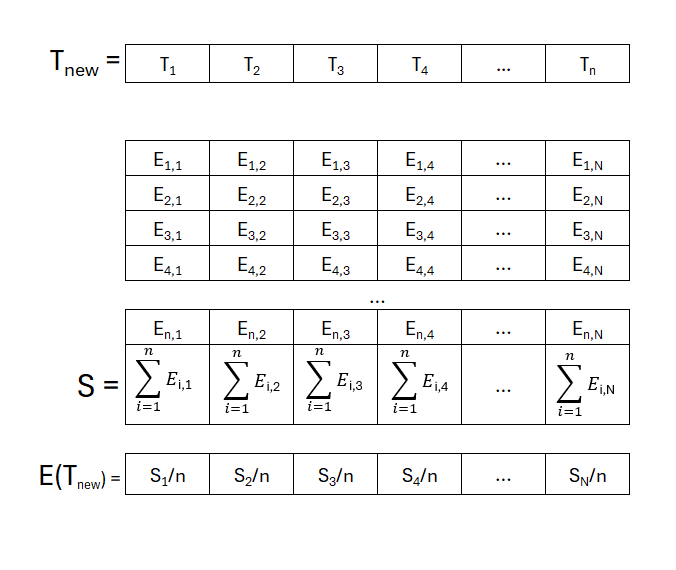
\includegraphics[width=0.5\linewidth]{Figures/mean_vector_embed_init.png}
%     \caption{Enter Caption}
%     \label{fig:placeholder}
% \end{figure}
% % ----------------------------------------------------------------------------------------



% ========================================================================================




% After computing the embeddings for all new tokens, the model's embedding matrix was extended by assigning:

% \begin{verbatim}
% model.embeddings.weight[new_token_id] = new_embedding_vector
% \end{verbatim}

% This method provides a straightforward approach that captures the average semantic content of the constituent tokens. The intuition behind this approach is that the meaning of a compound token can be approximated by the average meaning of its parts. For example, the Portuguese word "chegada" might be tokenized as "che" + "gada" in the original tokenizer, and the embedding for the new single token "chegada" would be the average of the embeddings for "che" and "gada".

% Although this approach is computationally efficient and intuitively sound, it treats all constituent tokens as equally important to the semantic meaning of the compound token, which may not always be the case, particularly in languages with complex morphological structures.




% \subsection{Position-Weighted Initialization}
% \label{subsec:pos-wei-init}
% The second approach, "Position-Weighted Initialization," assigns differential importance to constituent tokens based on their position within the sequence. This method is predicated on the hypothesis that initial tokens in a sequence typically carry greater semantic significance in autoregressive language models.

% For a new token decomposed into the sequence $(t_1, t_2, \ldots, t_n)$ by the original tokenizer, weights are assigned such that:

% $$
% \begin{array}{c}
%     \text{Let } new\_token = (t_1, t_2, \ldots, t_n) \\
%     E(new\_token) = \frac{\sum_{i=1}^{n} w_i \times E(t_i)}{\sum_{i=1}^{n} w_i} \\
%     \text{where } w_i = K^{n-i} \text{ for } i \in \{1,2,\ldots,n\}
% \end{array}
% $$

% The parameter $K > 1$ determines the degree of positional bias, with higher values of $K$ placing greater emphasis on earlier tokens. This approach was motivated by the observation that autoregressive models typically assign higher predictive importance to initial tokens in a sequence, and therefore the embedding should reflect this asymmetric relevance.

% For example, with $K = 1.5$ and a token decomposed into three subtokens, the weights would be approximately:
% \begin{itemize}
%     \item $w_1 = 1.5^2 = 2.25$ (first token)
%     \item $w_2 = 1.5^1 = 1.5$ (second token)
%     \item $w_3 = 1.5^0 = 1.0$ (third token)
% \end{itemize}

% All these weights are then normalized to sum to 1, resulting in:
% \begin{itemize}
%     \item $w_1 = \frac{2.25}{2.25+1.5+1} \approx 0.47$ (first token)
%     \item $w_2 = \frac{1.5}{2.25+1.5+1}  \approx 0.32$ (second token)
%     \item $w_3 = \frac{1}{2.25+1.5+1}    \approx 0.21$ (third token)
% \end{itemize}
% This weighting scheme ensures that the first token contributes more than twice as much to the final embedding as the last token, reflecting its greater importance in determining the semantic meaning of the compound token.

% \subsection{Comparative Analysis of Initialization Methods}
% We conducted extensive experiments to compare the effectiveness of these initialization strategies across various values of the weighting parameter $K$ for the Position-Weighted Initialization method. Figure \ref{fig:initialization_comparison} illustrates the performance of different initialization methods on the CalamePT benchmark.

% Empirical testing with various values of $K$ revealed that $K = 1.5$ provided optimal performance across evaluation metrics, balancing the influence of position while still incorporating information from all constituent tokens. Lower values of $K$ ($K < 1.3$) resulted in insufficient differentiation between token positions, while higher values ($K > 1.7$) placed too much emphasis on the initial tokens, effectively ignoring valuable information from later tokens.

% The Position-Weighted Initialization consistently outperformed the Mean Vector Initialization across all evaluation metrics, with an average improvement of 6.7 percentage points on the CalamePT benchmark and 3.3 percentage points on the SuperGluePTPT benchmark. This performance difference was particularly pronounced for longer compound tokens (those composed of 3 or more subtokens in the original tokenizer), where the position-weighted approach showed an average improvement of 9.2 percentage points.

% These results provide strong evidence for the importance of considering token position when initializing embeddings for new tokens, particularly in the context of autoregressive language models where the predictive distribution is conditioned on preceding tokens.


% \section{Embedding Fine-tuning}
% We also developed a method to fine-tune the embedding of a model for the newly added tokens.

% This was done by . . .  (include details on how this embedding training was calculated)







